\begin{remarkBox}{Intersections in Products}
    Intersection of rectangular sets behave nicely in products.
    Let \( A_{ 1 } \times \ldots \times A_{ r } \) and 
    \( B_{ 1 } \times \ldots \times B_{ r } \) be rectangular subsets of a 
    product of sets.
    Then
    \begin{equation*}
        ( A_{ 1 } \times \ldots \times A_{ r } ) 
        \cap 
        ( B_{ 1 } \times \ldots \times B_{ r } )
        =
        ( A_{ 1 } \cap B_{ 1 } ) \times \ldots \times ( A_{ r } \cap B_{ r } )
    \end{equation*}
    In particular, we have that an intersection of rectangular subsets is still
    rectangular.
    A similar equality holds for an \textit{arbitrary} intersection of
    rectangular subsets instead of just pairwise intersection.
\end{remarkBox}

\begin{remarkBox}{Unions in Products}
    Unlike with intersections, we \textit{cannot} just substitute \( \cap \)'s
    with \( \cup \)'s in the equality given for intersections in products.
    For example:
    \begin{equation*}
        ( \{ 0 \} \times \{ 0 \} )
        \cup 
        ( \{ 1 \} \times \{ 1 \} )
        \neq 
        ( \{ 0 \} \cup \{ 1 \} )
        \times
        ( \{ 0 \} \cup \{ 1 \} )
    \end{equation*}
    This is also evidence that a union of rectangular subsets need not be rectangular.

    \begin{figure}[H]
        \centering
        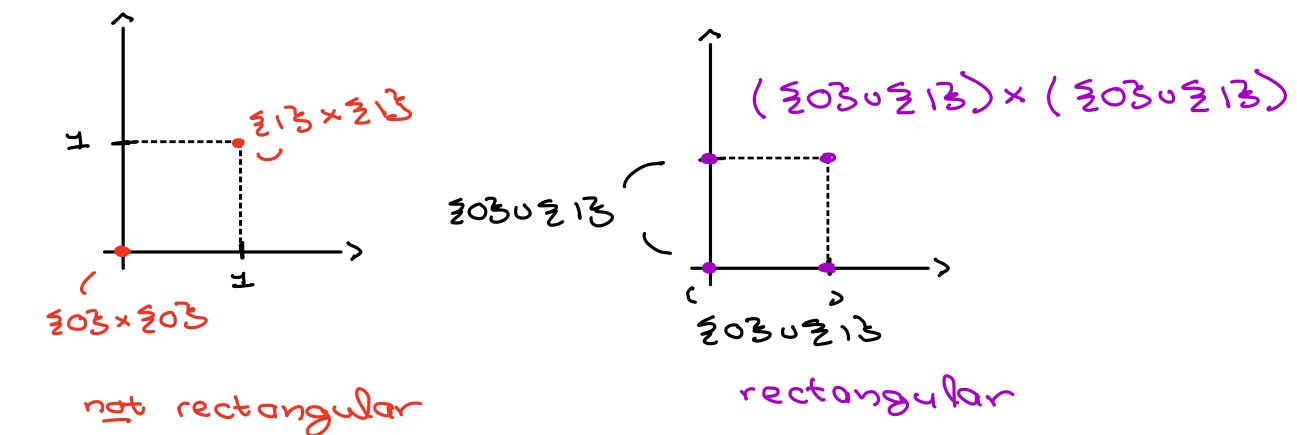
\includegraphics[ width = 0.5\linewidth ]{figures/Section 15/15_union.jpg}
        \caption{A visual of the example given}
        \label{fig:15-1}
    \end{figure}
\end{remarkBox}

\begin{remarkBox}{Complements in Products}
    Complements of rectangular subsets also behave a bit less nicely.
    For example:
    \begin{equation*}
        ( \mathbb{R} \times \mathbb{R} )
        \setminus
        ( \{ 0 \} \times \{ 0 \} )
        \neq 
        ( \mathbb{R} \setminus \{ 0 \} ) 
        \times 
        ( \mathbb{R} \setminus \{ 0 \} )
    \end{equation*}
    This is also evidence that a complement of rectangular subset need not be 
    rectangular.

    \begin{figure}[H]
        \centering
        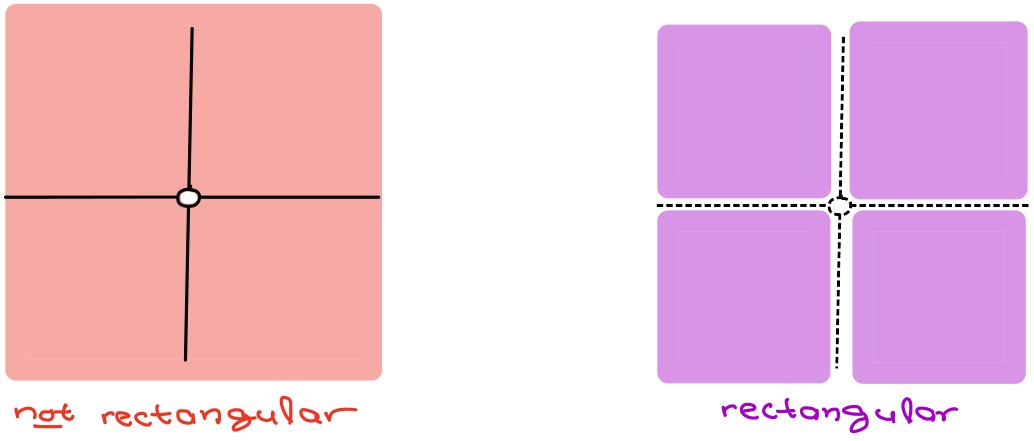
\includegraphics[ width = 0.5\linewidth ]{figures/Section 15/15_comp.jpg}
        \caption{A visual of the example given}
        \label{fig:15-2}
    \end{figure}

    The correct equality of rectangular subsets is as follows:
    \begin{equation*}
        ( X_{ 1 } \times \ldots \times X_{ r } )
        \setminus
        ( A_{ 1 } \times \ldots \times A_{ r } )
        =
        [ 
            ( X_{ 1 } \setminus A_{ 1 } ) \times X_{ 2 } 
            \times \ldots \times 
            X_{ r } 
        ]
        \cup \ldots \cup 
        [ 
            X_{ 1 } 
            \times \ldots \times 
            X_{ r - 1 } \times ( X_{ r } \setminus A_{ r } )
        ]
    \end{equation*}
    In fact, we see that this result holds for arbitrary products (since the proof
    only relies on DeMorgan's law, which works for arbitrary products).
\end{remarkBox}

\begin{remarkBox}{On the Basis for a Product Topology}
    It is important to note that the basis for a product topology is not a 
    topology on \( X \times Y \).
    For example take Figure (\ref{fig:15-3})

    \begin{figure}[H]
        \centering
        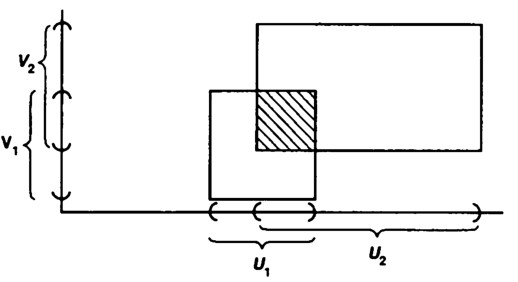
\includegraphics[ width = 0.5\linewidth ]{figures/Section 15/15_1.jpg}
        \caption{Visual of two open sets in \( X \) and \( Y \)}
        \label{fig:15-3}
    \end{figure}

    The union of the two rectangles in Figure (\ref{fig:15-3}) is not a product
    of two sets, so it cannot belong to \( \mathcal{B} \); however, we have that
    it is still open in \( X \times Y \) since for every point in the union, we
    can always find a smaller rectangle that is within the union that also
    contains our point.

    \baseSkip 
    However, the intersection of any two basic open sets is a basic open set.
\end{remarkBox}
